\section{Focal adhesion kinase}
Focal adhesions (FA) are macromolecular protein complexes which act as a connection hub between the cell, i.e. the cytoskeleton, and the extracellular matrix (ECM). They enable the cell to exert tension forces, but can also transduce mechanical stimuli from the ECM. One important protein associated to FA is the focal adhesion kinase (FAK). FAK occurs in several signalling pathways and is a key player in integrating extracellular stimuli. It is of large interest not least because in cancer cells often an overexpression of FAK can be found and understanding the activation processes and dynamics of FAK could give rise to new cancer treatments.% \autocite{cancerFAK}.
\subsection{Structure}
FAK consists of four domains: (i) a FERM domain at the N-terminus, (ii) a tyrosine kinase, (iii) a proline-rich region and (iv) a focal adhesion targeting (FAT) domain at the C-terminus (see \autoref{intro:fak}).\\
FERM (4.1 protein, ezrin, radixin and moesin) is a common protein domain which targets proteins to membranes \autocite{fermdomain} and consists of three subdomains: F1, F2 and F3. In the F2 subdomain a basic patch ($^{216}$KAKTLRK$^{222}$) can be found, which is a prominent binding site for phosphatidylinositol-4,5-bisphosphate (\pip, see below).\\
The kinase consists of the C-lobe, the activation loop and the N-lobe. Catalytic activity of kinase is mainly regulated by the phosphorylation of \acid{Y}{576}{} and \acid{Y}{577}, which are located in the activation loop \autocite{tyrosinePhosphor}. The kinase also provides binding sites for \pip{}. One important one is located next to the basic patch of the FERM domain, but others (namely \acid{R}{508}, \acid{R}{514}, \acid{K}{515}, \acid{K}{621} and \acid{K}{627}) can be found on the larger surface of the kinase \autocites{pap002}{pap002Exp}.\\
The FERM domain and the kinase are connected by a linker region. In contrast to other kinase domains, the main autophosphorylation site of FAK, \acid{Y}{397}, can be found in this region and not in the kinase itself \autocite{pap001}.\\ %TODO: better cite
The FAT domain is linked to the kinase by a flexible proline-rich region. FAT targets FA by interacting with talin and paxillin, which are proteins associated with FA \autocite{fatdomain}.
%
%
%
\begin{figure}
	\centering
	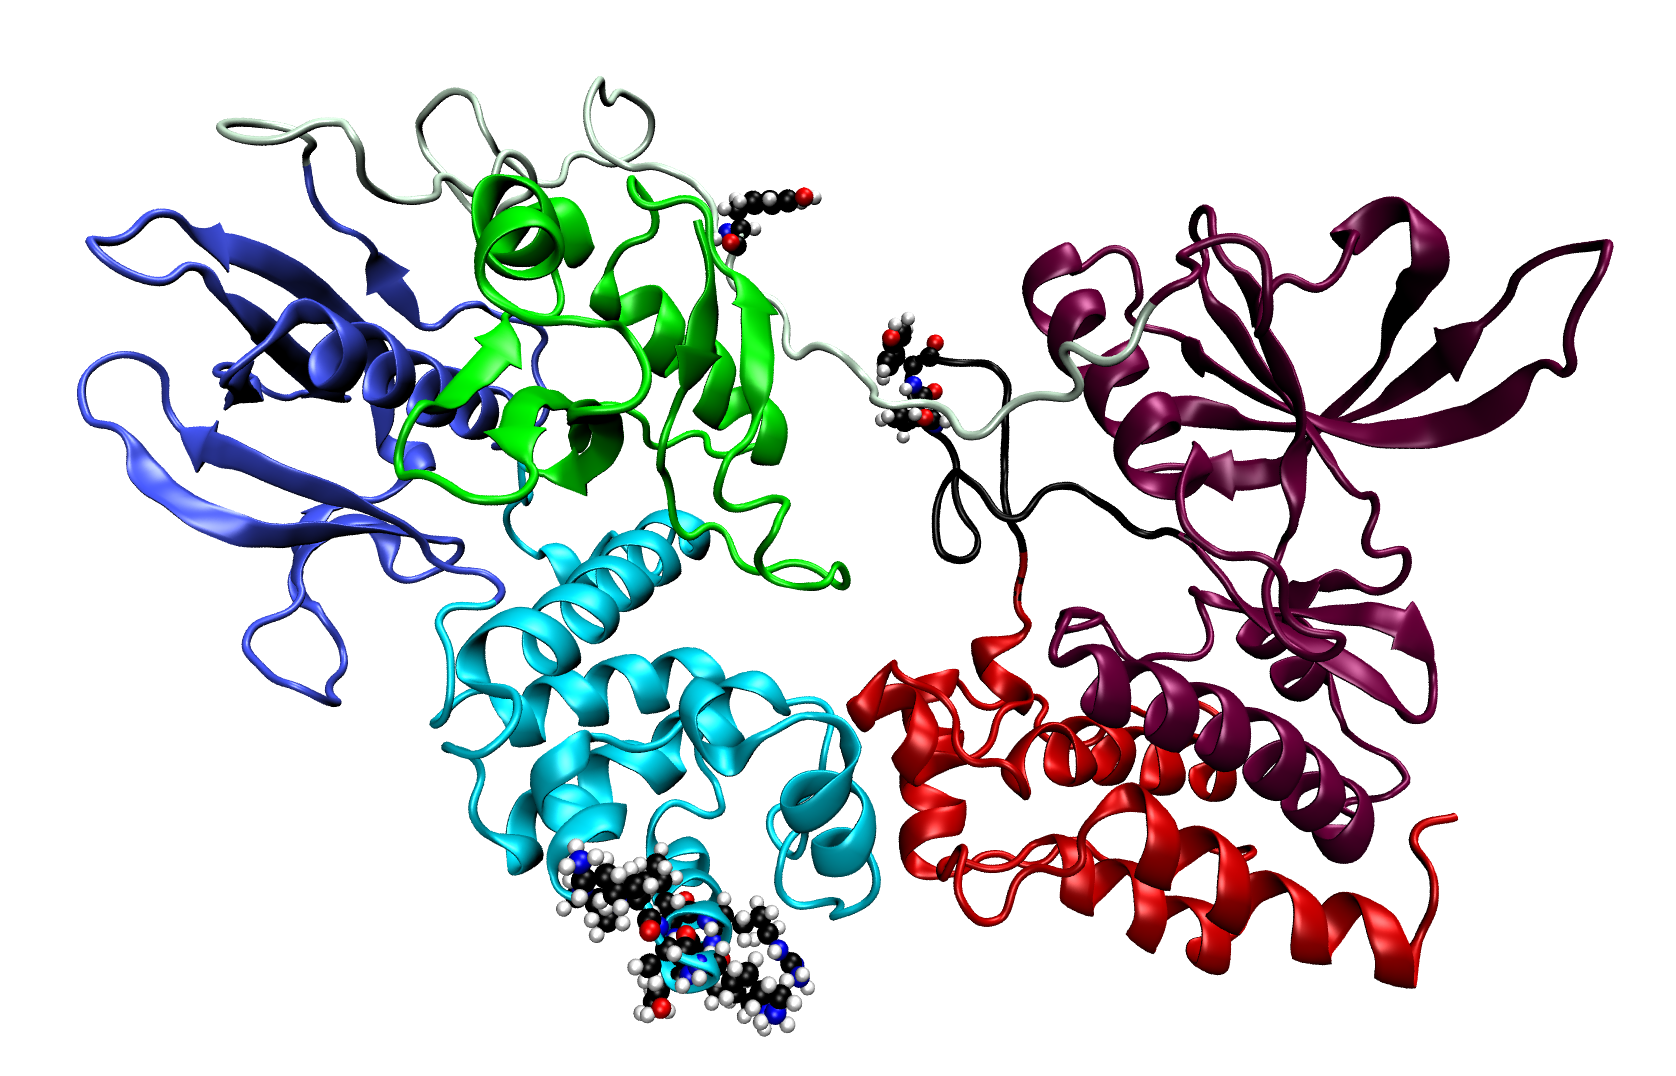
\includegraphics[height=6cm]{figures/introduction/fak}
	\nicecaption{Structure of FAK}{FERM domain consiting of F1 (green), F2 (iceblue) and F3 (blue) connected via the linker to the kinase consisting of N-lobe (violet), the activation loop (black) and the C-lobe (red). The basic patch (bottom), \acid{Y}{397} (top) and \acid{Y}{567}, \acid{Y}{577} (activation loop) are highlighted.}
	\label{intro:fak}
\end{figure}
%
%
%
\subsection{\pip{} binding and activation}
It is known that FAK triggers several stimuli. In this thesis, however, the focus is on the link of FAK activation and \pip{} binding. Therefore, the different binding sites of FAK for \pip{} and their impacts on FAK activation are discussed below.\\
\\
In the autoinhibited conformation described above, the FERM domain shields the active site of the kinase. An activation of FAK therefore requires the dissociation of these domains \autocite{structFAK}.\\
\pip{} is a phospholipid, which is locally generated in FA due to integrin signaling \autocite{CIT34}. 
%TODO: Add something on the pH-sensitivity of PIP2. It can be -3, -4, and -5 with various probabilities, strongly depending on the pH. 
It has a net charge of -4, but in presence of K the deprotonated state gets promoted resulting in a net charge of -5 \autocite{pip2_minus5}. The electrostatic binding of \pip{} to the basic patch in the F2 subdomain results in long ranged configurational changes, which also influence the interface between the F1 subdomain and the N-lobe. Also the linker region gets less strongly bound, so that an autophosphorylation of \acid{Y}{397} is promoted. However, the \pip{} binding alone has no effect on the catalytic activity, which suggests that the FERM domain is still associated to the kinase \autocites{pap001}{pap003}. For activation, an additional stimulus, either biochemical or mechanical, is needed.\\
\\
If \acid{Y}{397} is phosphorylated, it becomes a suitable binding site for SH2 or SH3, which are subdomains of proteins from the Src kinase family. Due to the conformational changes induced by \pip{}, this kinase has access to \acid{Y}{576} and \acid{Y}{577}. As said, the phosphorylation of these residues makes FAK fully active through a dissociation of the FERM domain and the kinase \autocite{pap001}.\\
\\
Another stimulus leading to the dissociation of the FERM domain from the kinase is mechanical force. Forces onto the FAT domain are transduced to the interface of the FERM domain and the kinase, because the linker is connected to the kinase, while the FERM domain is anchored onto a \pip{} containing membrane. These forces can lead to activation of FAK. In that way it is acting as an mechanical sensor \autocite{pap004}.\\
\\
The binding sites on the larger surface of the kinase were hypothesized by computer simulations \autocite{pap002} and have been confirmed recently in experiments \autocite{pap002Exp}. Their findings show that these residues are required for catalytic activity of the kinase, and that they bind to phospholipids \textit{in vivo}. However, since the catalytic activity is not regulated by \pip{}, this binding is supposed to act as a stabilisation of the active state on membranes only \autocite{pap002Exp}.
\subsection{Dimerization, clustering and autophosphorylation}
\label{intro:clustering}
As said above, autophosphorylation of \acid{Y}{397} is an important event in FAK activation. It has been shown that this happens in intact cell in \textit{in trans}, for which a self-association of FAK is required.\\
\\
The FERM domain induces a dimerization of FAK, as it is doing in other proteins containing a FERM domain as well. The interaction emerges around \acid{W}{266} in the connected FERM domains and is stabilised by an interaction of the FAT domain with the basic patch of the other FERM domain respectively. The presence of \acid{W}{266} is also required for autophosphorylation of FAK.\\
For the dimerization of the FERM domains \pip{} is not needed. However, an enriched concentration of FAK is needed to observe FAK dimers in cells, which is the case at FA. It is still unclear how the dimer is stabilized at membranes, where the basic patch is also required for ligand binding \autocite{fakdimers}.\\
It has been shown that FAK is autophosphorylated by other FAK molecules (intermolecular) and that this process is promoted by dimerization of FAK (not only due to FERM-FERM domains) \autocite{dimersVsClusters}.\\
\\
Although \pip{} is not required for dimerization, it induces clustering of several FAK \textit{in vitro} on membranes \autocite{pap001}. Because dimers support autophosphorylation of FAK, it is not surprising that the same effect is observed in clusters. However, these clusters can trigger additional biochemical stimuli \autocite{dimersVsClusters} and may play an important role in the scaffolding function of FAK for FA \autocite{pap001}.
